\documentclass[a4paper,12pt]{article}
\usepackage{times}
\usepackage{abakos}
\usepackage[hidelinks]{hyperref}
\providecommand{\htmladdnormallink}[2]{\href{#2}{#1}}

\makeatletter
\AddToHook{env/thebibliography/begin}{%
  \def\UrlLeft{}%
  \def\UrlRight{}%
  \urlstyle{same}%
}
\makeatother

\newcommand{\monog}{Teoria dos Grafos, Alta Performance e Observabilidade: análise comparativa de arquiteturas sob estresse de viralização}
\newcommand{\tipo}{Artigo}
\newcommand{\editorial}{}
\newcommand{\lcc}{{\scriptsize Licença Creative Commons Attribution-NonCommercial-NoDerivatives 4.0 International License}}

\newcommand{\AutorA}{Gabriel Assunção Costa}
\newcommand{\funcaoA}{}
\newcommand{\emailA}{}
\newcommand{\cursA}{Aluno do curso de Sistemas de Informação}
\newcommand{\AutorB}{Matheus Henrique Resende Magalhães}
\newcommand{\funcaoB}{}
\newcommand{\emailB}{}
\newcommand{\cursB}{Aluno do curso de Sistemas de Informação}

\newcommand{\univ}{Pontifícia Universidade Católica de Minas Gerais}
\newcommand{\keyword}[1]{\textsf{#1}}
\newcommand{\instrucao}{\color{blue}}
\newcommand{\estrutura}{\color{black}}
\usepackage{url}
\makeatletter
\g@addto@macro{\UrlBreaks}{\UrlOrds}
\makeatother
\usepackage{adjustbox}
\usetikzlibrary{arrows,shapes,positioning,shadows,trees}

\tikzset{
  basic/.style  = {draw, text width=3cm, drop shadow, font=\sffamily, rectangle},
  root/.style   = {basic, rounded corners=2pt, thin, align=center,
                   fill=blue!30},
  level 2/.style = {basic, rounded corners=6pt, thin,align=center, fill=green!30,
                   text width=8em},
  level 3/.style = {basic, thin, align=left, fill=pink!60, text width=6.5em}
}

\begin{document}
\begin{center}

\includegraphics[scale=0.25]{figuras/brasao} \\
PONTIFÍCIA UNIVERSIDADE CATÓLICA DE MINAS GERAIS \\
Instituto de Ciências Exatas e de Informática
\end{center}

\vspace{0cm}
{\singlespacing \Large{\monog \symbolfootnote[1]{Artigo apresentado ao Instituto de Ciências Exatas e Informática da Pontifícia Universidade Católica de Minas Gerais, campus Betim, como pré-requisito parcial para obtenção do título de Bacharel em Sistemas de Informação.} \\}}

\vspace{1.0cm}
\begin{flushright}
\singlespacing
\normalsize{\AutorA \footnote{\funcaoA \cursA.}} \\
\normalsize{\AutorB \footnote{\funcaoB \cursB.}}
\end{flushright}
\thispagestyle{empty}

\vspace{1.0cm}
\begin{abstract}
\noindent
\textcolor{blue}{O resumo é redigido em parágrafo único. Deve apresentar, de forma sucinta, o contexto, o problema, a justificativa, o objetivo, o desenvolvimento, os resultados e a conclusão do documento. O texto deverá conter de 100 a 250 palavras.}
\\\textbf{\keyword{Palavras-chave:}}
\end{abstract}

\selectlanguage{english}
\begin{abstract}
\noindent
\textcolor{blue}{The abstract must be written in a single paragraph and should briefly present the context, problem, justification, objective, development, results, and conclusion of the document. It should contain between 100 and 250 words.}
\\\textbf{\keyword{Keywords:}}
\end{abstract}

\selectlanguage{brazilian}
\onehalfspace
\setlength{\parindent}{1.25cm}
%%%%%%%%%%%%%%%%%%%%%%%%%%%%%%%%%%%%%%%%%%%%%%%%%%%%%%%%%%%%%%%%%%%%%%%%%%%%%%%%%%%%%%%%%%%%%%%%%%%%%%%
%%%%%%%%%%%%%% Template de Artigo Adaptado para Trabalho de Conclusão de Curso - SI Contagem - PUCMINAS %%%%%%%%%%%%%%%%%%%%%%%%
%% codificação UTF-8 - Abntex - Latex -  							     %%
%% Autor da primeira versão:    Fábio Leandro Rodrigues Cordeiro  (fabioleandro@pucminas.br)                            %% 
%% Co-autor da primeira versão: Prof. João Paulo Domingos Silva, Harison da Silva e Anderson Carvalho.                   %%
%% Revisores normas NBR (Padrão PUC Minas) da primeira versão: Helenice Rego Cunha e Prof. Theldo Cruz.                   %%
%% Versão: 1.1     18 de dezembro de 2015 
%% Revisora normas NBR (Padrão PUC Minas) da terceira versão: Profa. Amália Vasconcelos.                   %%
%% Versão: 3.0     02 de fevereiro de 2026  
%%%%%%%%%%%%%%%%%%%%%%%%%%%%%%%%%%%%%%%%%%%%%%%%%%%%%%%%%%%%%%%%%%%%%%%%%%%%%%%%%%%%%%%%%%%%%%%%%%%%%%%%%%%%%%%%%%%%%%%%%%%%%%%%
\estrutura\section{\esp Introdução}

Redes sociais permitem que conteúdos se propaguem rapidamente entre usuários e produzam variações intensas no volume de interação. A disseminação decorre das características do conteúdo e das decisões sucessivas de compartilhá-lo, enquanto a posição do usuário na rede condiciona o alcance potencial de cada publicação. Quando um conteúdo alcança usuários com grande capacidade de disseminação, compartilhamentos sucessivos podem gerar picos de requisições, processamento e persistência. A estrutura dessas cascatas não se reduz ao total de compartilhamentos, pois a dinâmica também varia ao longo da propagação \cite{liang2021,sepehr2022}. A teoria dos grafos permite representar as relações entre usuários, identificar posições estruturalmente relevantes e descrever esse processo. Neste trabalho, a rede social será modelada como um grafo dirigido, e o grau de saída será adotado como medida operacional do alcance potencial dos iniciadores, sem pressupor equivalência com influência efetiva \cite{zareie2023}. As cascatas serão representadas separadamente, por meio dos usuários que compartilharam o conteúdo e das exposições que antecederam cada compartilhamento. Essa representação orientará a geração de cargas que considerem o volume, a distribuição e a evolução temporal dos eventos.

O problema desta pesquisa consiste em investigar como diferentes arquiteturas \textit{backend} respondem ao estresse gerado por cascatas de informação em redes sociais. A investigação é orientada pela seguinte pergunta: como a topologia da rede e a concentração de influência em nós com alto grau de saída afetam o desempenho, a formação de filas, a utilização de recursos e a resiliência de duas composições arquiteturais, uma predominantemente síncrona e outra orientada a eventos, quando submetidas ao mesmo padrão simulado de viralização? A comparação considera uma arquitetura síncrona, baseada em PHP-FPM, Laravel e MySQL, com fluxo síncrono e persistência transacional linha a linha, e uma arquitetura orientada a eventos, baseada em PHP com Swoole/Hyperf, RabbitMQ e Neo4j, com processamento assíncrono, filas e ingestão em lotes por \textit{workers}.

A relevância do estudo está em aproximar propriedades estruturais da rede das consequências observáveis na infraestrutura de software. Medidas como alcance, profundidade, largura e velocidade descrevem aspectos dependentes entre si e, por isso, requerem controle conjunto na comparação de cascatas \cite{juul2021}. Além disso, formas distintas de difusão podem produzir padrões diferentes de requisições e escritas persistentes \cite{sepehr2022}. A avaliação conjunta de grafos, carga e observabilidade pode, portanto, oferecer uma análise experimental mais precisa da degradação e da resiliência das arquiteturas, sem restringir a comparação ao tempo de resposta nem pressupor a superioridade de uma composição.

O objetivo geral é analisar comparativamente o comportamento de duas composições arquiteturais completas, uma síncrona e outra orientada a eventos, durante a simulação de cascatas de informação associadas à viralização em redes sociais. O estudo não busca isolar o efeito individual de cada tecnologia, mas comparar as composições sob condições equivalentes de carga. Para alcançá-lo, são definidos os seguintes objetivos específicos: i) modelar redes e cascatas com diferentes distribuições de conectividade e concentrações de grau de saída; ii) implementar geradores de carga capazes de reproduzir picos controlados de compartilhamento; iii) submeter as duas arquiteturas ao mesmo estímulo; iv) coletar métricas de recursos, latência, \textit{throughput}, erros, filas, persistência e rastreamento distribuído; e v) comparar saturação, degradação, drenagem das filas e recuperação após o pico. Os parâmetros e critérios que assegurarão a equivalência dos experimentos serão definidos na metodologia antes de sua execução.

O restante deste artigo está organizado da seguinte forma: o referencial teórico define os conceitos de redes, cascatas, arquiteturas e observabilidade empregados na pesquisa; a seção de trabalhos relacionados examina estudos próximos à comparação proposta; a metodologia descreve a classificação da pesquisa, o desenho experimental, o modelo de carga e os procedimentos de coleta e análise dos dados; a seção de desenvolvimento apresenta a implementação das arquiteturas e dos mecanismos de simulação e observabilidade; os resultados apresentam e discutem os dados obtidos nos experimentos; e, por fim, as considerações finais sintetizam as conclusões, as limitações e as possibilidades de trabalhos futuros.

\estrutura\section{\esp Referencial Teórico}

Esta seção reúne os conceitos necessários para relacionar a estrutura das redes sociais ao comportamento das duas composições arquiteturais sob carga. A exposição parte da representação da rede e da propagação da informação, caracteriza os fluxos síncrono e orientado a eventos e, por fim, delimita os sinais e indicadores usados para observar a resposta dos sistemas.

\estrutura\subsection{\esp Redes sociais e teoria dos grafos}

Um grafo é uma estrutura formada por vértices e arestas: no domínio deste estudo, cada vértice representa um usuário e cada aresta dirigida representa uma relação pela qual um conteúdo pode alcançar outro usuário. O grau de um vértice corresponde ao número de arestas que incidem nele; em grafos dirigidos, o grau de saída contabiliza as conexões que partem do usuário. Redes que crescem por conexão preferencial podem concentrar muitas relações em poucos vértices, produzindo distribuições desiguais de conectividade \cite{piva2021}. A centralidade designa uma família de medidas empregadas para caracterizar a posição estrutural dos vértices. Neste trabalho, o grau de saída será uma variável operacional de centralidade, e o alcance indicará quantos usuários podem ser atingidos a partir de um iniciador. Influência, por sua vez, será entendida como a capacidade efetiva de induzir comportamentos, não como sinônimo automático de conectividade, pois atributos comportamentais e o modelo de difusão também afetam a propagação \cite{zareie2023}.

Propagação é o processo pelo qual a informação percorre as relações da rede. Uma cascata de informação é o subgrafo formado pelos compartilhamentos de um conteúdo e pelas exposições que os antecedem. Sua profundidade é a maior distância, em gerações de compartilhamento, entre o iniciador e um participante; sua largura corresponde à quantidade de ocorrências em uma mesma geração. O alcance contabiliza os participantes ou expostos, enquanto a forma da cascata distingue, por exemplo, uma difusão ampla e rasa de outra distribuída por várias gerações. Essa distinção é necessária porque cascatas de tamanhos semelhantes podem possuir estruturas e mecanismos de difusão diferentes \cite{sepehr2022,juul2021}.

\estrutura\subsection{\esp Viralização e efeito manada}

Viralização corresponde, neste trabalho, à disseminação rápida e ampla de um conteúdo por sucessivos compartilhamentos. O chamado efeito manada descreve a tendência de uma pessoa adotar um comportamento após observar a adesão de outras, de modo que a exposição social pode alterar a probabilidade de compartilhar. A posição topológica do iniciador condiciona o público que pode ser alcançado, mas métricas puramente estruturais não explicam, isoladamente, a decisão de retransmitir. Estudos recentes mostram que fatores relacionados ao usuário, à mensagem e à geração da cascata modificam os efeitos de contágio, inclusive com variação ao longo da profundidade \cite{liang2021}; por isso, alto grau de saída será tratado como alcance potencial, e não como prova de influência.

A literatura também adverte que tamanho, profundidade, largura e evolução temporal não devem ser interpretados como dimensões independentes. O pareamento apenas pelo tamanho pode ocultar diferenças relevantes na estrutura das cascatas \cite{juul2021}, enquanto medidas de virulência estrutural procuram representar como a difusão se distribui entre transmissões diretas e sucessivas gerações \cite{sepehr2022}. Assim, a carga experimental deverá controlar tanto o volume total quanto a distribuição temporal e topológica dos eventos. O uso do termo efeito manada, portanto, não pressupõe que toda exposição resulte em adesão; ele delimita o mecanismo social simulado que poderá produzir concentração de eventos em curto intervalo.

\estrutura\subsection{\esp Arquitetura síncrona}

Na comunicação síncrona por requisição e resposta, um cliente envia uma solicitação e aguarda a conclusão do processamento para receber o resultado. Revisões sobre padrões de comunicação em microsserviços distinguem esse acoplamento temporal dos padrões assíncronos e mostram que a escolha do padrão depende do contexto e de seus desafios operacionais \cite{aksakalli2021}. Na primeira composição deste estudo, o PHP-FPM gerencia processos FastCGI em grupos de \textit{workers}, com modos configuráveis de criação de processos e informações de estado apropriadas à operação sob carga \cite{phpfpm2026}. O Laravel recebe a requisição, aplica as regras da operação e coordena o acesso ao MySQL antes de produzir a resposta.

A persistência relacional organiza os dados em tabelas e relacionamentos definidos por chaves. A expressão ``linha a linha'' identifica que cada evento de compartilhamento gera operações individuais de inserção ou atualização, ainda que várias operações possam pertencer à mesma transação. Uma transação delimita uma unidade de trabalho concluída por confirmação, que torna permanentes as alterações, ou por reversão, que as cancela \cite{mysql2026}. Nessa composição, o tempo percebido pelo cliente inclui o processamento da aplicação e a persistência necessária à resposta; sob aumento de concorrência, requisições podem aguardar processos, conexões ou recursos do banco. Essas relações constituem hipóteses a observar, não resultados antecipados.

\estrutura\subsection{\esp Arquitetura orientada a eventos}

Em uma arquitetura orientada a eventos, mudanças relevantes são representadas como eventos e publicadas para processamento por componentes desacoplados no tempo. Swoole fornece ao PHP um mecanismo de rede baseado em eventos assíncronos e corrotinas, sobre o qual o Hyperf estrutura a aplicação \cite{swoole2026}. O produtor cria a mensagem; o RabbitMQ atua como intermediador e a armazena em uma fila; o consumidor a recebe; e um \textit{worker}, isto é, um processo responsável por executar unidades de trabalho, realiza o processamento. A requisição pode terminar depois da aceitação do evento, sem aguardar toda a persistência subsequente, razão pela qual latência de aceitação e latência de processamento completo deverão ser medidas separadamente.

Processamento assíncrono significa que produção e consumo não precisam ocorrer simultaneamente. Quando a chegada supera temporariamente a capacidade dos consumidores, mensagens pendentes formam um \textit{backlog}. O processamento em lote agrupa várias mensagens em uma operação de persistência, reduzindo a quantidade de interações com o banco, mas introduzindo critérios de tamanho e tempo para formar cada lote. No RabbitMQ, a confirmação do consumidor informa que uma entrega foi processada, enquanto a confirmação do publicador indica que o intermediador assumiu responsabilidade pela mensagem; são mecanismos distintos e necessários à definição explícita da confiabilidade \cite{rabbitmq2026}.

O Neo4j representa entidades como nós e relações como conexões de primeira classe. Nesta composição, usuários e compartilhamentos podem ser persistidos segundo a topologia que será percorrida nas análises. Operações no grafo, nos índices ou no esquema ocorrem em transações, e atualizações muito grandes precisam ser divididas para limitar o consumo de memória \cite{neo4j2026}. A ingestão em lotes não elimina, portanto, a fronteira transacional: ela altera a quantidade de eventos reunidos em cada unidade de persistência. A comparação será feita entre composições completas, sem atribuir antecipadamente eventual diferença a uma tecnologia isolada.

\estrutura\subsection{\esp Observabilidade sob carga}

Observabilidade é a capacidade de inferir o estado interno de um sistema a partir dos sinais que ele produz. Métricas são séries numéricas agregadas; \textit{logs} são registros discretos de eventos com seu contexto; e rastreamento distribuído acompanha uma operação pelas etapas e componentes que a processam. A correlação temporal e por identificadores entre esses sinais permite relacionar alterações de desempenho a requisições, mensagens, \textit{workers} e operações de persistência \cite{tzanettis2022}. O OpenTelemetry será empregado como estrutura independente de fornecedor para gerar, coletar e exportar esses sinais, sem substituir os sistemas responsáveis por armazená-los e visualizá-los \cite{opentelemetry2026}.

Sob carga, latência é o tempo transcorrido para concluir uma operação, e vazão é a quantidade de operações concluídas por unidade de tempo. Como médias podem ocultar ocorrências extremas, percentis como p50, p95 e p99 indicarão os limites abaixo dos quais se encontram, respectivamente, 50\%, 95\% e 99\% das observações. A taxa de erros expressará a proporção de operações malsucedidas; saturação caracterizará o ponto em que um recurso se aproxima de sua capacidade e o aumento de demanda passa a intensificar espera ou falhas. Na composição assíncrona, o tamanho do \textit{backlog} quantificará mensagens ainda não concluídas e o tempo de drenagem medirá o intervalo necessário para processar a fila remanescente após o encerramento do pico. Esses indicadores, juntamente com CPU, memória e duração da persistência, são variáveis planejadas para os experimentos e não constituem resultados já obtidos.

\estrutura\section{\esp Trabalhos Relacionados}

\citeonline{abella2023} analisaram o efeito do envelhecimento dos agentes na dinâmica temporal de cascatas por meio de um modelo de limiar para contágio complexo. O método incorporou diferentes mecanismos de envelhecimento e avaliou como eles alteram a evolução macroscópica do processo. O estudo contribui ao distinguir as condições de ocorrência da cascata de sua velocidade de propagação. Assim como este TCC, considera que a distribuição temporal dos eventos é relevante; diferentemente dele, concentra-se na dinâmica do modelo social, e não na resposta de arquiteturas \textit{backend} ao padrão de carga resultante.

\citeonline{cabane2024} compararam empiricamente versões monolítica e orientada a eventos de uma mesma aplicação, submetendo-as a cargas e analisando CPU, memória, tempo de resposta, vazão e tráfego de rede. A contribuição está na avaliação conjunta de métricas e no tratamento estatístico das diferenças observadas. A semelhança com este TCC é a comparação experimental de composições arquiteturais sem pressupor superioridade de um estilo; a diferença está no estímulo, pois o presente estudo empregará cascatas derivadas de propriedades topológicas e também observará filas, drenagem e rastros distribuídos.

\citeonline{kotiranta2022} compararam Neo4j, MySQL e MariaDB por meio de consultas com estruturas e complexidades distintas, considerando também índices e otimizações. O trabalho contribui ao demonstrar que o desempenho depende do tipo de consulta e da configuração, sem sustentar a superioridade universal de um modelo de dados. A semelhança está na presença de persistência relacional e orientada a grafos; a diferença é que o presente TCC avaliará ingestão durante cascatas de carga em arquiteturas completas, e não o desempenho isolado de consultas entre bancos.

Em síntese, os três estudos oferecem fundamentos para controlar a dinâmica temporal, comparar estilos arquiteturais e interpretar diferenças entre bancos. No conjunto selecionado, entretanto, não foi identificada uma avaliação que transforme propriedades topológicas de cascatas sociais em estímulo controlado para comparar uma composição síncrona e outra orientada a eventos. Este trabalho busca atender a essa lacuna ao relacionar a propagação simulada aos sinais de infraestrutura, sem antecipar resultados nem atribuir eventual comportamento a uma tecnologia isolada.

\iffalse

%\textcolor{red}{\textbf{Importante:}} mantenha atualizada a versão do TeX Live. No Overleaf, escolha o "motor" de compilação no menu \texttt{File >\allowbreak\ Settings >\allowbreak\ Compiler >\allowbreak\ TeX Live version >\allowbreak\ selecione a mais atual}. Ex.: 2025.

A formatação deverá ter parágrafo recuado a 1,25 cm, tamanho 12, fonte Arial ou Times New Roman, espaçamento entre linhas de 1,5 cm e texto justificado. Os títulos dos capítulos devem utilizar a formatação caixa alta, negrito, tamanho 12. As seções e subseções devem seguir às normas ABNT, como pode ser observado ao longo deste documento. Nesse sentido, este template já possui a formatação correta com margens, espaçamentos e tipo de folha requisitada no TCC. Quanto ao limite de páginas exigido no trabalho, são no mínimo 11 (onze) e no máximo 15 (quinze) páginas, incluindo referências, anexos e apêndices.

A introdução deve conter 1 - 2 páginas e ser apresentada em texto contínuo. Ainda que existam partes com funções distintas, o texto deve manter encadeamento lógico. Cada parágrafo deve corresponder a um dos tópicos indicados a seguir, sem subtítulos, ou seja, sem a utilização explícita de termos como, por exemplo, contexto, problema, justificativa, entre outros.

	Contexto. Descrever o tema/área em que o trabalho se insere. 
	Ex.: a ocorrência de problemas psicológicos entre os adolescentes tem levado os educadores a se preocuparem com a possibilidade de que o mal uso das novas tecnologias possa estar provocando danos aos mesmos. A preocupação é agravada diante da constatação de que a maior parte dos adolescentes tem livre acesso aos conteúdos disponíveis na web \cite{citelli2004,martins2012}.
	
 Problema. Qual pergunta o seu trabalho procura responder? 
	Ex.: a inclusão digital nem sempre é realizada por meio das escolas, portanto ela pode ocorrer de uma forma não estruturada e sem o acompanhamento necessário. Mas mesmo quando a introdução às tecnologias, principalmente a informática, é realizada nas escolas, pode ocorrer o uso das mesmas pelos adolescentes sem o devido controle, fora das escolas. Como então a informática tem influenciado no processo de formação dos adolescentes?
	
 Justificativa. Por que essa pergunta é importante? Quais os benefícios você trará ao resolver este problema?
	Ex.: ao determinar-se a influência da informática no processo de formação dos adolescentes, é possível elaborar estratégias de ensino que aproveitem as habilidades adquiridas pelos adolescentes para uma utilização correta e efetiva das tecnologias. Também pode-se identificar as dificuldades encontradas pelos adolescentes no uso da tecnologia e promover o aprendizado nas escolas, visando mitigar tais dificuldades.
	
 Objetivo. O que você fará neste trabalho? Como vai resolver o problema?
	Ex.: o objetivo geral deste trabalho é analisar a influência da informática no processo de formação de adolescentes, utilizando um estudo de caso fundamentado na aplicação de questionários sobre inclusão digital.
	
 Objetivos específicos. São detalhamentos do objetivo geral, que descrevem metas intermediárias a serem cumpridas para que o objetivo geral seja atingido.
	Ex.: já os objetivos específicos deste trabalho são: i) identificar escolas públicas de ensino médio na região metropolitana de Belo Horizonte, que ofereçam disciplinas introdutórias de informática na grade curricular; ii) caracterizar o perfil socioeconômico dos estudantes das escolas identificadas...
	
 Estrutura do trabalho. Descrever cada seção do seu trabalho.	
	Ex.: este texto está estruturado em 5 seções. A seção 2 apresenta o referencial teórico… A seção 3 descreve os trabalhos relacionados. Na seção 4… Por último, ...


\estrutura\section{\esp Referencial Teórico (2 - 3 páginas)}\instrucao

Todo título de seção ou subseção deverá ser seguido de texto.  Para criar uma seção use \verb|\section{}|, e para as subseções use \verb|\subsection{}| e \verb|\subsubsection{}|. A ABNT permite até cinco níveis de subseções, no entanto, evite mais de dois níveis para melhor organização e fluidez do texto.


O Referencial Teórico é organizado no formato de uma pirâmide. No topo, o tópico mais abrangente. Na base, o tópico mais específico. Ou seja, escreve-se menos sobre o tópico mais abrangente e mais sobre o tópico específico. Ex.: nesta seção são descritos os principais conceitos, classificações e técnicas relacionados a inclusão digital. 

\estrutura\subsection{\esp Tópico mais abrangente (Ex.: Inclusão digital)}\instrucao 
\label{subsec:1}
Por exemplo, para descrever o que é computação paralela, deve-se apresentar, pelo menos, três referências diferentes e escrever um parágrafo, com as suas próprias palavras, que resuma o que foi entendido das referências. Deve-se produzir um texto contínuo, de forma que as referências estejam concatenadas entre si.

As citações das referências podem ser diretas ou indiretas. As referências deverão ser adicionadas no arquivo \textit{bibliografia.bib}. Cada referência deverá ser adicionada conforme o padrão de normalização da PUC, 
o qual poderá ser consultado na página da biblioteca da \citeonline{manualpuc2025}. Todas as publicações citadas no texto deverão ter correspondente nas referências, 
e as indicações de autoria da citação e do ano deverão ser idênticas aos dados expostos. 

Para adequar-se à nova norma ABNT NBR 10520:2023, que não utiliza mais citações em caixa-alta, não exclua o arquivo \textit{abntex2-alf.bst} do seu projeto no Overleaf. É importante ressaltar que algumas entradas ainda podem apresentar inconformidades, como ao usar o comando \verb|\cite{}| para referências que possuem o campo \verb|@organization| preenchido, mas não têm o campo \verb|@author| ou o campo \verb|@editor| preenchido. A comunidade \texttt{abntex} está trabalhando em uma solução definitiva para esses casos. 

\estrutura\subsection{\esp Tópico intermediário (Ex.: Inclusão informacional) }\instrucao
O mesmo procedimento descrito na Seção \ref{subsec:1} deve ser aplicado a cada parágrafo do capítulo do referencial teórico.

\estrutura\subsection{\esp Tópico específico (Ex.: Inclusão social) }\instrucao
O mesmo procedimento descrito na Seção \ref{subsec:1} deve ser aplicado a cada parágrafo do capítulo do referencial teórico.




\estrutura\subsection{\esp Elementos flutuantes}\instrucao

São elementos inseridos no texto como imagens, tabelas, algoritmos, etc.
De acordo com as normas ABNT, há a necessidade de se observar que todos os elementos flutuantes inseridos devem ter a formatação básica:

\begin{enumerate} [label={\alph*})]
 \item título centralizado localizado na parte superior; 
 \item fonte em tamanho 10 na parte inferior;
 \item se o elemento for de autoria própria, siga o exemplo do Quadro \ref{qua:quadro1}; caso contrário, faça a citação da referência conforme o exemplo da Figura \ref{fig:figura1}. Para elementos criados a partir de outros autores, usar a expressão  ``Adaptado de ...'' 
 \item devem ser inseridos o mais próximo do texto que os referenciam.
\end{enumerate}


\estrutura\subsubsection{\esp Inserções de ilustrações}\instrucao

As ilustrações devem ser inseridas seguindo o exemplo da Figura \ref{fig:figura1}. Nos casos de telas de software, estas também devem ser inseridas como figuras, e referenciadas no texto. Além disso, é necessário que seja citada no texto a empresa desenvolvedora, quando aplicável. 

% Figura
\begin{figure}[ht]
	\centering	
	\caption{Uma grade computacional como fonte transparente}
	\vspace{-0.4cm}
	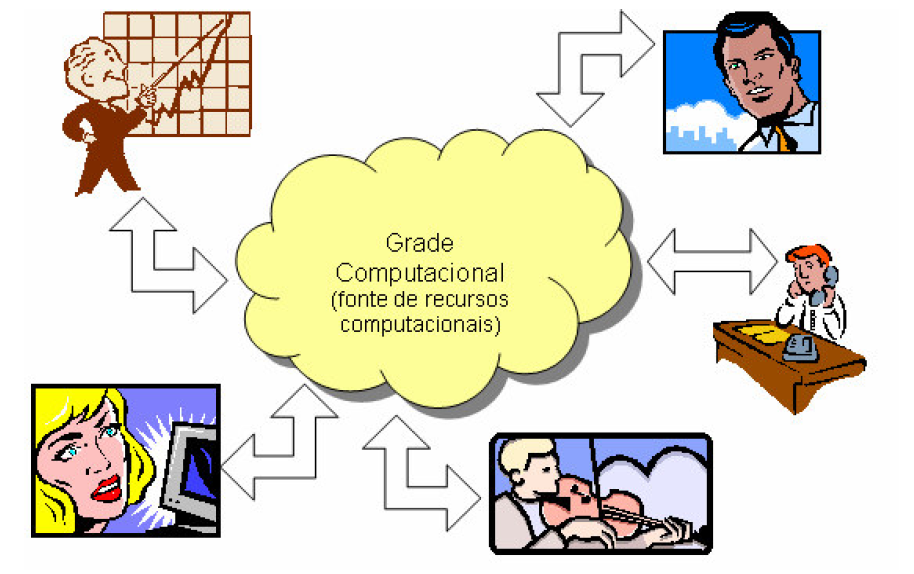
\includegraphics[width=0.7\textwidth]{figuras/grade-comp.png}
	% Caption centralizada
% 	\captionsetup{justification=centering}
	% Caption e fonte 
	 \vspace{-0.2cm}
	\\\textbf{\footnotesize Fonte: \citeonline{cap-livro2005} }
	\label{fig:figura1}
\end{figure}
\vspace{-0.5cm}

   \newpage

 \subsubsection{\esp Tabelas}

As tabelas devem ser abertas nas laterais, com espaços verticais separando
as colunas e sem espaços horizontais, exceto na
separação do cabeçalho. Um exemplo é a Tabela \ref{tab:tabela1}: 

% Tabela
\begin{table}[htb]
	\centering
	\caption{Exemplo de uma tabela}
	\vspace{-0.3cm} % espaço entre titulo e tabela
	\label{tab:tabela1}
	% Conteúdo da tabela
	\begin{tabular}{l|c|c}
  \hline
    \textbf{Imagem}	& \textbf{Transferência} & \textbf{Tempo} \\
    \hline
     estação 1	& 7,72 MB/s &  1:22:18 \\
     estação 2	& 7,72 MB/s &  1:22:17 \\
     estação 3	& 7,59 MB/s & 1:24:25 \\
     estação 4  & 7,53 MB/s & 1:43:27 \\
     estação 5	& 6,14 MB/s  &  1:24:41 \\
     estação 6  &  7,50 MB/s & 1:23:53 \\
     estação 7  & 7,58 MB/s  &  1:24:02 \\
     estação 8  & 7,8 MB/s  &  1:29:06 \\
     estação 9  & 7,9 MB/s  &  1:30:05 \\
     estação 10 & 8,0 MB/s  &  1:32:03 \\
     \hline
 \end{tabular}
 	\vspace{.1cm}  %espaço entre tabela e fonte
	\small
	% Fonte
	{\footnotesize\\ \textbf{Fonte: \citeonline{monografia2010}}}
\end{table}

\estrutura\subsubsection{\esp Quadros}\instrucao

Os quadros diferem das tabelas por apresentarem dados textuais.
Esses dados podem ser esquemáticos, comparativos ou descritivos.
  	
   	\begin{quadro}[H]
   		\centering
   		\caption{Bandas/Artistas de Rock e outros}
   	\label{qua:quadro1}
   		% Conteúdo do quadro
	\begin{tabular}{|c|c|c|c|} \hline
	\multicolumn{4}{|c|}{\textbf{Bandas ou Artistas de Rock e outros}} 	  \\ 
		\hline \textbf{	Progressivo} & Pink Floyd & Jethro Tull	& Yesterday \\ 
		 \hline \textbf{ Metal}  & Metallica & Iron Maidam & Black Sabath \\ 
		\hline \textbf{	Arena Rock} & Led Zeppelin & The Rolling Stones & Beatles \\ 
		\hline \textbf{ Punk} & Ramones & Black Flag & NOFX	\\ 
		\hline \textbf{	Nacional} & Ira & Engenheiros & Vinil	\\ 
		\hline \textbf{	S.J.E.} & Apolo XI & Invasão 7 & Por do Sol \\ 
		\hline \textbf{	Grunge} & Nirvana & Pear Jam & Alice in Chains	\\ 
		\hline \textbf{	Rock Folk} & Bod Dylan & The Byrds &  The Mamas \& the Papas \\
		\hline \textbf{	Blues} & B.B. King & Albert Colins & Mady Wathers \\ 
		\hline \textbf{	New Wave} & The Police & The Pretenders, &  Duran Duran\\ 
 		\hline \textbf{	Rock Folk} & Bod Dylan & The Byrds &  The Mamas \& the Papas \\
 		\hline \textbf{	Rock alternativo} & R.E.M.& Hüsker Dü & Big Black\\ 
		\hline
	\end{tabular}
	\vspace{.1cm}  %espaço entre quadro e fonte
	\small
	% Fonte
	{\footnotesize\\ \textbf{Fonte: Elaborado pelo autor}}
   \end{quadro}

   
\estrutura\subsubsection{\esp Inserção de algoritmos}\instrucao

Para inserir um algoritmo, utilizar o exemplo do Algoritmo  \ref{alg:rnagenerica}.
Todos os algoritmos devem ser inseridos assim como é feito para figuras, tabelas, ou seja, devem ser indicados por nome e fonte.


\begin{center}	
    \textbf{Algoritmo 1 -  CAC RD Neural}
	\vspace{-0.3cm}
\begin{minipage}[ht]{13cm}
\begin{algorithm}[H]
  \footnotesize
  \caption{CAC-RD Neural}
  \label{alg:rnagenerica}
  \begin{algorithmic}[1]
      \STATE \textbf{Entrada:} Requisição da chamada
    \STATE \textbf{Saída:} Aceitação ou bloqueio da solicitação
    
    \STATE Preenche o vetor de $attributes.size+1$ atributos com os valores dos atributos, sendo a primeira posição do vetor preenchida com o valor 1
		\STATE $hidden\_layer\_size =  attributes.size*2+1;$

    \FOR{$i$ = 1 to $attributes.size+1$}
    	\STATE \textbf{normalizar}($Entrada_i$)
    \ENDFOR

		\STATE $double [] net = new double [hidden\_layer\_size];$
    \STATE $net = hidden\_layer\_weights * attributes;$
   	\FOR{$i$ = 0 to hidden\_layer\_size}
			\STATE $net [i] = 1.0 / (1.0 + exp((-1.0)*net[i]));$
		\ENDFOR

		\STATE $double [] ipVector = new double [hidden\_layer\_size+1];$
    \STATE $ipVector [0] = 1.0;$
   	\FOR{$i$ = 1 to $hidden\_layer\_size+1$}
			\STATE $ipVector [i] = net [i-1];$
		\ENDFOR
		
		\STATE $output = output\_layer\_weights *  ipVector;$
    \STATE output = \textbf{desnormalizar}(Saída)
    \STATE \textbf{net\_update} (requisition);
    
    \STATE \textbf{Retorna} output; FIM
  \end{algorithmic}
\end{algorithm}
% \vspace{-0.3cm} % espaço entre algoritmo e fonte

\small \centering \textbf{\footnotesize Fonte: \citeonline{mestrado2010}.}
\end{minipage}
\end{center}
% \end{figure}
   
\estrutura\section{\esp Trabalhos Relacionados (1 página)}\instrucao

A seção de Trabalhos Relacionados deve apresentar um pequeno resumo (um parágrafo) de cada artigo, monografia ou demais trabalhos que tenham feito algo parecido com o seu trabalho. Em seguida, devem ser destacadas as diferenças e semelhanças entre o seu trabalho e o relacionado. Devem ser apresentados no mínimo 3 trabalhos relacionados. Os trabalhos relacionados não devem ter sido usados como referências no capítulo anterior. Recomenda-se que esta seção seja sustentada por literatura recente, priorizando publicações dos últimos cinco anos.

Lembre-se de usar corretamente a formatação para citações. As citações podem ser classificadas como livres, diretas ou citação de citação, esta última não abordada neste documento.


\estrutura\subsection{\esp Citação livre ou indireta}\instrucao

Quando se reproduzir ideias, sem transcrever as palavras do autor, a indicação da página é opcional. Exemplos desse tipo de citação:
\begin{enumerate} 
 \item citação com um autor \cite{knuth1968}. 
 \item citação de artigos em revistas com dois autores \cite{prenner2022}.\footnote{Quando citar um artigo, inclua o DOI (Identificador de Objeto Digital) sempre que estiver disponível.}
  \item trabalho em congresso com três autores \cite{vasconcelos2016}.
 \item trabalhos com mais de três autores \cite{cap-livro2005}.
 \item citação de dois autores de uma vez em duas obras distintas \cite{gil2022,groupp2003}.
\end{enumerate}

\estrutura\subsection{\esp Citação direta ou textual}\instrucao

Transcrição literal de textos de outros autores. Nesse caso, deverão ser especificadas as páginas consultadas. 


\estrutura\subsubsection{\esp Textual curtas}\instrucao

Quando curtas (até 3 linhas) serão inseridas na sequência normal do texto, entre aspas duplas com as mesma formatação.

\estrutura\subsubsection{\esp Textual longas}\instrucao

Citações longas (mais de 3 linhas) deverão constituir um parágrafo independente, recuado a 4 cm da margem esquerda, 
com letra tamanho 10 e digitado em espaço simples, sem aspas.
\begin{citacaodireta}
Hegel chama trabalho à forma específica da satisfação das necessidades, que
distingue da natureza o espírito existente. Assim como a linguagem infringe
a imposição da intuição e ordena o caos das múltiplas sensações em coisas
identificáveis, assim o trabalho infringe a imposição do \hspace{0.1cm}desejo \hspace{0.1cm}imediato \hspace{0.1cm}e
suspende, por assim dizer, o processo de satisfação das necessidades.
\cite[25]{habermas1997}.
\end{citacaodireta}


\instrucao
% Artigo \cite{whatershed:01}

\estrutura\subsubsection{\esp Textual de outros idiomas (tradução)}\instrucao

Quando a citação estiver em outro idioma e for traduzida, indique após a chamada da citação a expressão tradução nossa ou tradução própria, entre parênteses. Obs: Em nota de rodapé informe, se desejar, a citação direta no idioma consultado.

\begin{citacaodireta} 
Um cluster é um computador paralelo construído de componentes e processos de software (tal como sistema de software). 
Um cluster é formado de nós, cada um contendo um ou mais processadores, memória que é compartilhada por todos os processadores do nodo 
(somente eles), e dispositivos periféricos adicionais (tais como discos), conectados pela rede e que permitem tráfego de dados entre os nós...
\cite[p. 10, tradução nossa]{groupp2003}\footnote {... a cluster is a parallel computer that is constructed of commodity  components and runs 
(as its system software) commodity software. A cluster is made of nodes, each 
containing one or more processors, memory that is  shared 
by all of the processors in (and only on) the node, and additional peripheral devices (such as disks), connected by network that allows data to move between the nodes.}.
\end{citacaodireta}
 
\estrutura\subsection{\esp Exemplos de citações}\instrucao 

Seguem alguns exemplos de citações mais utilizadas e/ou que geram algumas dúvidas. É válido observar que não serão citadas aqui
todas as possibilidades de citações. Sendo assim é de extrema relevância que se consulte o documento no site da Biblioteca (\citeonline{manualpuc2025}) para maiores esclarecimentos acerca de citações.

\estrutura\subsubsection{\esp Citação de monografia, dissertação e tese}\instrucao

Um exemplo de citação de monografia de curso de graduação ou especialização pode ser visto em \citeonline{monografia2010}.
Já para dissertação de mestrado veja \citeonline{mestrado2010}. E para o doutorado a citação é feita da seguinte forma: \citeonline{tese2012}. 



\estrutura\subsubsection{\esp Livros e partes de livros}\instrucao

Exemplo de capítulo de livro fica conforme esse exemplo: \citeonline{cap-livro2005}.

Para livros citados no corpo do texto e com duas citações juntas, ver os exemplos: \citeonline{knuth1968,groupp2003}.

\fi

\iffalse
\newpage

\estrutura\section{\esp Metodologia (1 - 2 páginas)}\instrucao
A Metodologia descreve o tipo e as etapas da pesquisa, estabelecendo um plano detalhado para a coleta e análise de dados. Além disso, uma metodologia bem definida permite a replicação do estudo, contribui para a transparência dos procedimentos e facilita a interpretação e aplicação dos achados.

    \subsection{\esp Classificação da pesquisa}
As pesquisas podem ser classificadas de diversas formas, como pode ser visualizado na Figura \ref{fig:metodologia}. Para mais informações sobre tais classificações, consulte materiais como \citeonline{gil2022,wazlawick2021}.

\begin{figure}[H]
    \centering
    \caption{Classificação das pesquisas científicas \citeonline{gil2022}}
    \begin{adjustbox}{valign=c}
		\resizebox{0.85\textwidth}{!}{ % para ajustar o tamanho da figura
    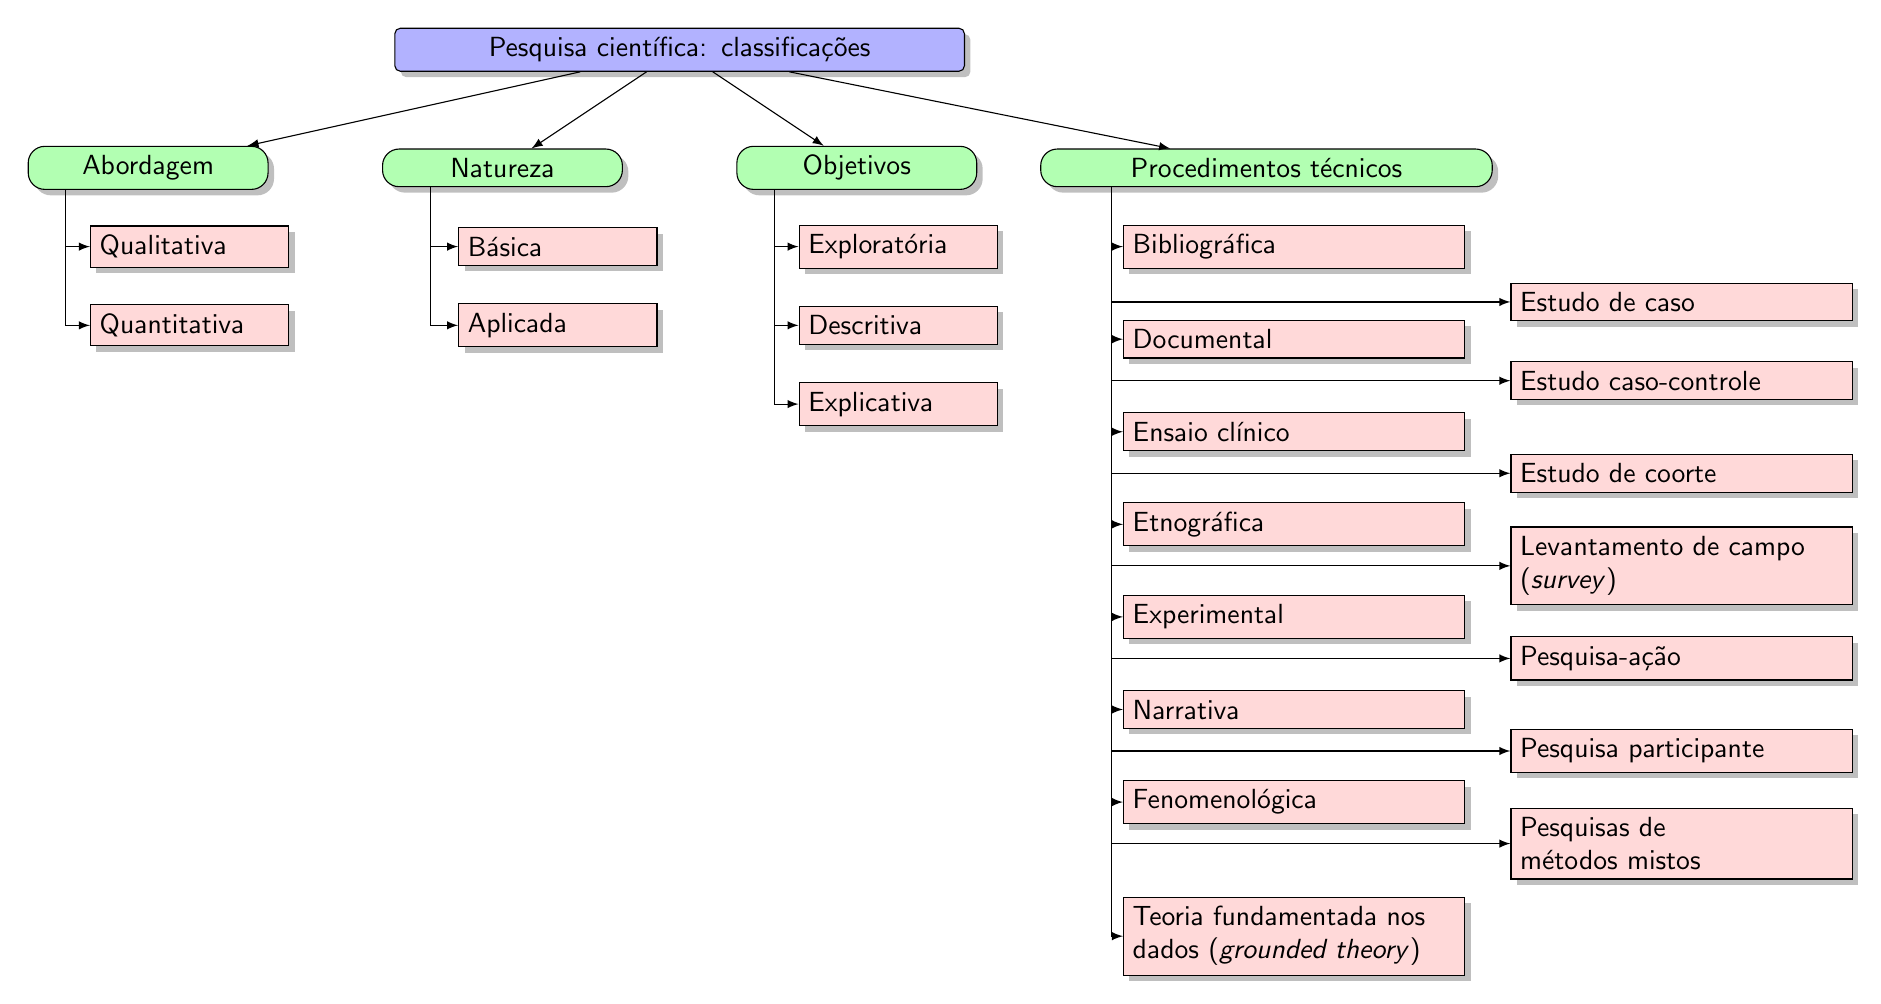
\begin{tikzpicture}[
  level 1/.style={sibling distance=45mm},
  edge from parent/.style={->,draw},
  >=latex]

% root of the the initial tree, level 1
\node[root,text width=7cm] {Pesquisa científica: classificações}
% The first level, as children of the initial tree
  child {node[level 2] (c1) {Abordagem}}
  child {node[level 2] (c2) {Natureza}}
  child {node[level 2] (c3) {Objetivos}}
  child {node[level 2, xshift=20pt, text width=5.5cm] (c4) {Procedimentos técnicos}};
;

% The second level, relatively positioned nodes
\begin{scope}[every node/.style={level 3}]
\node [below of = c1, xshift=15pt] (c11) {Qualitativa};
\node [below of = c11] (c12) {Quantitativa};

\node [below of = c2, xshift=20pt] (c21) {Básica};
\node [below of = c21] (c22) {Aplicada};

\node [below of = c3, xshift=15pt] (c31) {Exploratória};
\node [below of = c31] (c32) {Descritiva};
\node [below of = c32] (c33) {Explicativa};
\node [below of = c4, xshift=10pt, text width=4.1cm] (c41) {Bibliográfica};
\node [below of = c41, yshift=-5pt, text width=4.1cm] (c42) {Documental};
\node [below of = c42, yshift=-5pt, text width=4.1cm] (c43) {Ensaio clínico};
\node [below of = c43, yshift=-5pt, text width=4.1cm] (c44) {Etnográfica};
\node [below of = c44, yshift=-5pt, text width=4.1cm] (c45) {Experimental};
\node [below of = c45, yshift=-5pt, text width=4.1cm] (c46) {Narrativa};
\node [below of = c46, yshift=-5pt, text width=4.1cm] (c47) {Fenomenológica};
\node [below of = c47, yshift=-20pt, text width=4.1cm] (c48) {Teoria fundamentada nos dados (\textit{grounded theory})};
\node [below of = c4, xshift=150pt, yshift=-20pt, text width=4.1cm] (c49) {Estudo de caso};
\node [below of = c49, yshift=0pt, text width=4.1cm] (c410) {Estudo caso-controle};
\node [below of = c410, yshift=-5pt, text width=4.1cm] (c411) {Estudo de coorte};
\node [below of = c411, yshift=-5pt, text width=4.1cm] (c412) {Levantamento de campo (\textit{survey})};
\node [below of = c412, yshift=-5pt, text width=4.1cm] (c413) {Pesquisa-ação};
\node [below of = c413, yshift=-5pt, text width=4.1cm] (c414) {Pesquisa participante};
\node [below of = c414, yshift=-5pt, text width=4.1cm] (c415) {Pesquisas de \linebreak métodos mistos};
\end{scope}



% lines from each level 1 node to every one of its "children"
\foreach \value in {1,2}
  \draw[->] (c1.195) |- (c1\value.west);

\foreach \value in {1,...,2}
  \draw[->] (c2.195) |- (c2\value.west);

\foreach \value in {1,...,3}
  \draw[->] (c3.195) |- (c3\value.west);

 \foreach \value in {1,...,15}
   \draw[->] (c4.195) +(-30pt,0) |- (c4\value.west);
\end{tikzpicture}}
\end{adjustbox}
	\vspace{.1cm}  %espaço entre figura e fonte
	\\\textbf{\footnotesize Fonte: Elaborada pelo autor}  
 \label{fig:metodologia}
\end{figure}

É importante esclarecer em quais tipos de pesquisa o seu estudo se enquadra.
Ex.: este trabalho caracteriza-se como uma pesquisa de abordagem quantitativa, de natureza aplicada, com objetivos descritivos e explicativos, uma vez que busca mensurar e analisar o comportamento de determinadas variáveis por meio de dados numéricos. A coleta de dados foi realizada por meio de questionários estruturados, cujos resultados foram submetidos a tratamento estatístico, incluindo cálculos de frequência, medidas descritivas e métricas de desempenho, possibilitando a análise objetiva dos fenômenos investigados. Quanto aos procedimentos técnicos, o estudo pode ser classificado como um estudo de caso.

\estrutura\subsection{\esp Etapas da pesquisa}\instrucao

	Nesta subseção, deve-se descrever as etapas para a realização da pesquisa. Como foi identificada e selecionada a amostra? Como foi feita a elaboração e aplicação dos questionários da pesquisa? Cada etapa deve ser detalhada.

Ex.: esta pesquisa é dividida nas seguintes etapas:

\begin{enumerate}
\item levantamento bibliográfico;
\item elaboração de questionários;
\item estruturação e definição das entrevistas;
\item aplicação dos questionários e entrevistas;
\item apresentação, interpretação e análise dos resultados obtidos.
\end{enumerate}

Na elaboração dos questionários, foram levantados os principais fatores que podem influenciar na formação dos adolescentes e as ferramentas possivelmente utilizadas. Para cada um desses fatores, foram elaboradas questões de múltipla escolha e abertas. O questionário foi respondido por 30 pessoas, sendo 10 pessoas de cada classe social (baixa, média e alta). A determinação de classe social foi feita utilizando-se o Critério Brasil de Classificação Social.


\estrutura\subsection{\esp Ambiente de desenvolvimento}\instrucao
Caso o escopo do trabalho envolva o desenvolvimento de software, é indispensável descrever o ambiente de desenvolvimento utilizado. Ex.: Neste trabalho, o ambiente de desenvolvimento é constituído pelas ferramentas e tecnologias apresentadas no Quadro \ref{qua:quadro2}.

\begin{quadro}[H]
    \centering
    \caption{Ferramentas e tecnologias do ambiente de desenvolvimento}
    \label{qua:quadro2}
    \begin{tabular}{|C{4.5cm}|C{4.5cm}|C{3cm}|}
    \hline
    \textbf{Categoria} & \textbf{Ferramenta} & \textbf{Versão} \\ \hline
    Backend e API       & .NET 8 / ASP.NET Core & 8.0 (LTS)     \\ \hline
    Frontend web        & React.js / Next.js    & 18.2 / 14.1   \\ \hline
    Banco de dados      & PostgreSQL            & 16.1          \\ \hline
    Desenvolvimento mobile & Flutter            & 3.19          \\ \hline
    Conteinerização     & Docker Containers     & 24.0.x        \\ \hline
    Monitoramento       & Grafana / Prometheus  & 10.x / 2.x    \\ \hline
    Sistema operacional & Windows 11 / Linux    & 23H2 / Ubuntu \\ \hline
    \end{tabular}
    \vspace{.1cm} 
    \small
    {\footnotesize\\ \textbf{Fonte: Elaborado pelo autor}}
\end{quadro}


\estrutura\section{\esp Desenvolvimento (2 - 3 páginas)}\instrucao
Se o escopo do trabalho envolver o desenvolvimento de software, esta seção deve detalhar o processo de construção, desde o levantamento de requisitos até a implementação.

\estrutura\subsection{Levantamento de requisitos}\instrucao
Nesta etapa, devem ser descritos os requisitos funcionais e não funcionais do sistema. Ex.: após a análise dos sistemas de aula virtual existentes e das necessidades da proposta, os requisitos funcionais (RF) foram definidos conforme o Quadro \ref{qua:quadro3}.

\begin{quadro}[H]
    \centering
    \caption{Requisitos funcionais do sistema}
    \label{qua:quadro3}
    \begin{tabular}{|C{2cm}|C{12.5cm}|}
    \hline
    \textbf{ID} & \textbf{Descrição do requisito} \\ \hline
    RF01 & Permitir que o usuário visualize vídeos das aulas por módulo. \\ \hline
    RF02 & Permitir que o usuário responda questionários de múltipla escolha. \\ \hline
    RF03 & Disponibilizar a emissão de certificados após a conclusão do curso. \\ \hline
    \end{tabular}
    \vspace{.1cm} 
    \small
    {\footnotesize\\ \textbf{Fonte: Elaborado pelo autor}}
\end{quadro}

Da mesma forma, os requisitos não funcionais (RNF) que regem os atributos de qualidade do software estão apresentados no Quadro \ref{qua:quadro4}.

\begin{quadro}[H]
    \centering
    \caption{Requisitos não funcionais do sistema}
    \label{qua:quadro4}
    \begin{tabular}{|C{2.5cm}|C{12.5cm}|}
    \hline
    \textbf{ID / Tipo} & \textbf{Descrição do requisito} \\ \hline
    RNF01 (Desempenho) & O sistema deve suportar até 60 alunos simultâneos sem perda de desempenho. \\ \hline
    RNF02 (Segurança) & O acesso às funcionalidades deve ser restrito via autenticação de login e senha. \\ \hline
    RNF03 (Usabilidade) & A interface deve seguir princípios de design responsivo para dispositivos móveis. \\ \hline
    \end{tabular}
    \vspace{.1cm} 
    \small
    {\footnotesize\\ \textbf{Fonte: Elaborado pelo autor}}
\end{quadro}

\estrutura\subsection{Modelagem do sistema}\instrucao
Nesta subseção, apresenta-se o diagrama de casos de uso. Deve-se apresentar também o diagrama de classes ou o modelo de entidade-relacionamento (MER). 

Ex.: a Figura \ref{fig:caso_uso} mostra as interações do aluno com o sistema.

% Figura
\begin{figure}[H]
	\centering	
    \caption{Diagrama de caso de uso do ator aluno}
   % \vspace{-0.4cm}
	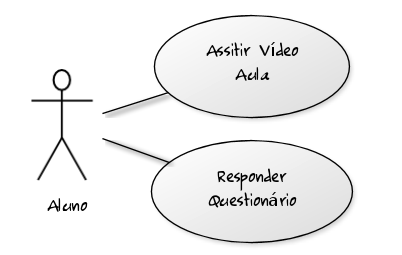
\includegraphics[width=0.5\textwidth]{figuras/caso_uso.png}
	% Caption centralizada
% 	\captionsetup{justification=centering}
	% Caption e fonte 
	 \vspace{-0.2cm}
	\\\textbf{\footnotesize Fonte: Elaborada pelo autor}
    \label{fig:caso_uso}
\end{figure}
\vspace{-0.5cm}


\estrutura\subsection{Interface do sistema}\instrucao
Apresentar e descrever as principais telas da interface do sistema.

\estrutura\section{\esp Resultados (2 - 3 páginas)}\instrucao

Nesta seção, devem ser apresentados os dados coletados, acompanhados de suas respectivas análises. Caso o trabalho envolva o uso de métodos quantitativos, é aqui que devem ser inseridos os testes estatísticos, cálculos de variância, correlação ou significância.

Nos Resultados você deve apresentar os gráficos com os resultados obtidos e também analisá-los. Note que apresentar é apenas descrever o que pode ser visto no gráfico, enquanto que analisar significa explicar o porquê dos resultados apresentados (essa explicação deve ser sustentada por dados da pesquisa. Caso não seja, deve-se deixar claro que se trata se uma possibilidade não comprovada).


Ex.: o Quadro \ref{qua:quadro5} apresenta a quantidade de adolescentes que utilizam computador nas escolas. Pode-se observar que todos os alunos da classe alta utilizam computadores na escola, comparado com apenas 30\% dos alunos da classe baixa. (apresentação)

\begin{quadro}[H]
   		\centering
   		\caption{Quantidade de adolescentes que utilizam computador nas escolas}
   	\label{qua:quadro5}
   		% Conteúdo do quadro
\begin{tabular}{|c|C{3cm}|C{3cm}|}
\hline
\multirow{2}{*}{\textbf{Classe}} & \multicolumn{2}{c|}{\textbf{Você utiliza computador na escola?}} \\ \cline{2-3} 
                                 & \textbf{Sim} & \textbf{Não} \\ \hline
Baixa                            & 3            & 7            \\ \hline
Média                            & 8            & 2            \\ \hline
Alta                             & 10           & 0            \\ \hline
\end{tabular}
	\vspace{.1cm}  %espaço entre quadro e fonte
	\small
	% Fonte
	{\footnotesize\\ \textbf{Fonte: Elaborado pelo autor}}
   \end{quadro}

Exemplo de análise e dados estatísticos: na classe média, constatou-se que 20\% dos alunos não utilizam computadores no ambiente escolar. Tal resultado decorre do fato de que esses estudantes frequentam instituições públicas sem laboratórios ativos. Ao aplicar o teste de correlação (estatística), verificou-se que o acesso à tecnologia é diretamente proporcional à classe socioeconômica, com um p-valor < 0,05, indicando significância estatística nos dados apresentados.

Além disso, nos Resultados devem ser apresentadas métricas relacionadas ao sistema. Em trabalhos que envolvem classificação ou predição, também devem ser apresentadas métricas de avaliação. Da mesma forma, nesta seção devem ser descritos e analisados os testes de software realizados. A apresentação desses resultados deve evidenciar o atendimento aos requisitos e objetivos do trabalho, sendo sempre acompanhada de análise crítica fundamentada nos dados obtidos durante os experimentos e testes realizados.

\estrutura\section{\esp Considerações Finais (1 página)}\instrucao


É o capítulo de encerramento do trabalho, que contém a discussão dos resultados obtidos na pesquisa. É onde se colocam as observações do autor.  A conclusão deve estar de acordo com os objetivos do trabalho. Ela não deve apresentar citações ou interpretações de outros autores.

Sendo assim, a conclusão é composta pelos seguintes elementos, os quais devem ser apresentados em texto corrido. Cada parágrafo deve corresponder a um dos tópicos indicados a seguir, sem o uso de subtítulos, ou seja, sem a utilização explícita de termos como, por exemplo, conclusão geral, discussão dos resultados, contribuições da pesquisa ou trabalhos futuros.

	Conclusão Geral. Síntese do que foi realizado. Os objetivos foram alcançados totalmente? Os resultados foram compatíveis com as expectativas?
	Ex.: este trabalho apresentou um estudo de caso da inclusão digital de adolescentes, realizado por meio da análise de questionários, que foram aplicados para identificação da influência da informática no processo de formação destes adolescentes. Os resultados mostram que os adolescentes de classe baixa com acesso a informática ainda são uma minoria.
	
 Discussão dos Resultados. Extrapolação dos resultados obtidos (e se...); destaque das limitações, vantagens e desvantagens da pesquisa, entre outras observações.
	Ex.: nesta pesquisa não foi analisado o impacto da informática na formação de crianças e jovens. Apesar disso, os resultados poderiam ser estendidos para estas diferentes faixas etárias.
	
 Contribuições da Pesquisa. Metas alcançadas, ou seja, os objetos importantes produzidos.
	Ex.: a principal contribuição desta pesquisa foi identificar que adolescentes são excluídos do mundo digital principalmente pela falta de aulas de informática nas escolas públicas, independente da classe econômica.
	
 Trabalhos Futuros. Possíveis evoluções da pesquisa, sugestões de pesquisas relacionadas etc.
	Ex.: como trabalhos futuros, pretende-se realizar um estudo de caso do impacto da informática na formação de crianças e jovens. Além disso, pretende-se fazer um estudo sobre a inclusão digital mais restrita aos adolescentes estudantes de escolas públicas.
\fi


\newpage
\estrutura
\singlespace{
\renewcommand\refname{REFERÊNCIAS}
\bibliography{bibliografia}
}
\bibliographystyle{abntex2-alf}
\end{document}
